\documentclass{article}
\usepackage{tikz}
\begin{document}
\begin{flushleft}
Find the shortest paths, and their lengths, from vertex \textit{$v_1$} to each of the other vertices in the graph shown below. \textit{(Weights appear off the centre point of corresponding edge.)}
\end{flushleft}
\begin{center}
\begin{tabular}{ |c||c|c|c|c|c|}
\hline
 & \textit{$v_{1}$} & \textit{$v_{2}$} & \textit{$v_{3}$} & \textit{$v_{4}$} & \textit{$v_{5}$}\\
\hline\hline
\textit{$v_{1}$} & 0& 11& 0& 5& 9\\
\hline
\textit{$v_{2}$} & 11& 0& 0& 0& 0\\
\hline
\textit{$v_{3}$} & 0& 0& 0& 10& 4\\
\hline
\textit{$v_{4}$} & 5& 0& 10& 0& 3\\
\hline
\textit{$v_{5}$} & 9& 0& 4& 3& 0\\
\hline
\end{tabular}
\end{center}
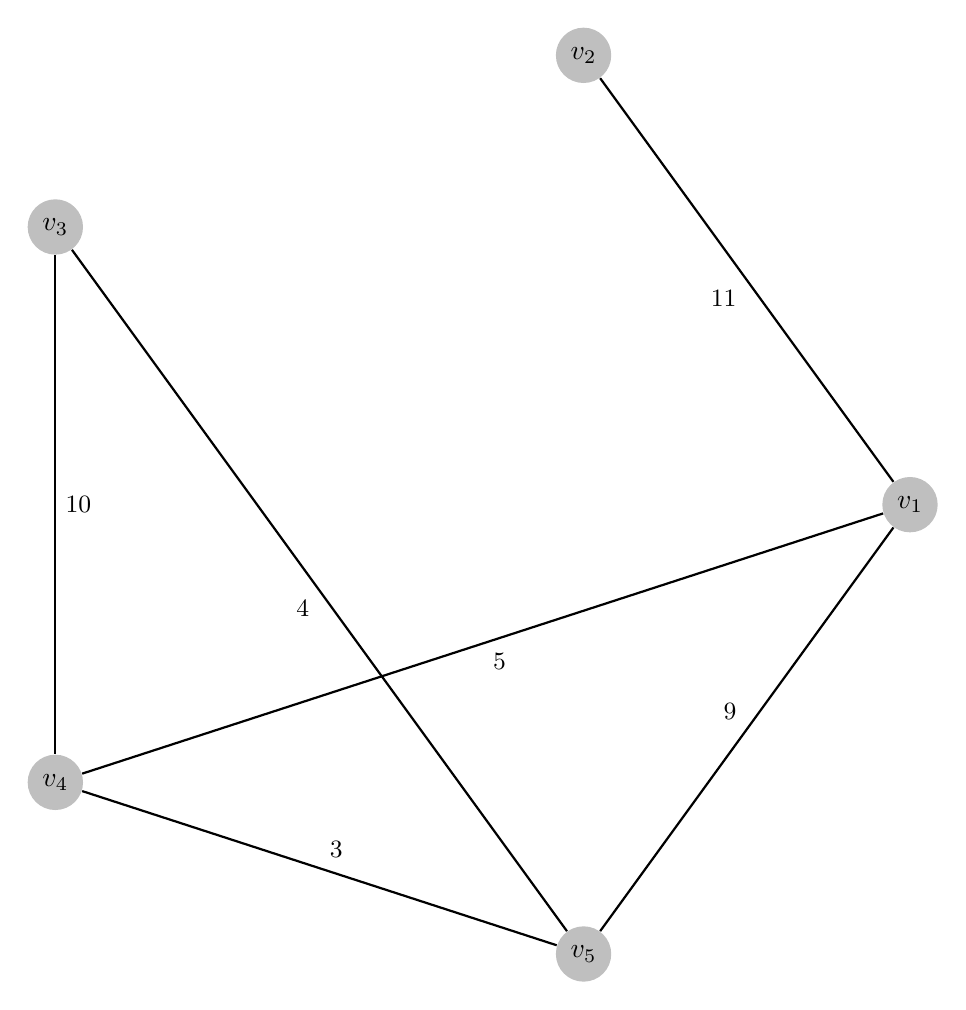
\begin{tikzpicture}[auto]
\tikzstyle{vertex}=[circle,fill=black!25,minimum size=20pt,inner sep=0pt]
\tikzstyle{edge} = [draw,thick,-]
\tikzstyle{weight} = [font=\small]
\def \radius {6cm}
\node[vertex] (1) at ({360/5 * (0 )}:\radius) {$v_{1}$};
\node[vertex] (2) at ({360/5 * (1 )}:\radius) {$v_{2}$};
\node[vertex] (3) at ({360/5 * (2 )}:\radius) {$v_{3}$};
\node[vertex] (4) at ({360/5 * (3 )}:\radius) {$v_{4}$};
\node[vertex] (5) at ({360/5 * (4 )}:\radius) {$v_{5}$};
\path[edge] (1) -- node[weight] {$11$} (2);
\path[edge] (1) -- node[weight] {$5$} (4);
\path[edge] (3) -- node[weight] {$10$} (4);
\path[edge] (4) -- node[weight] {$3$} (5);
\path[edge] (5) -- node[weight] {$9$} (1);
\path[edge] (5) -- node[weight] {$4$} (3);
\end{tikzpicture}
\end{document}
